
	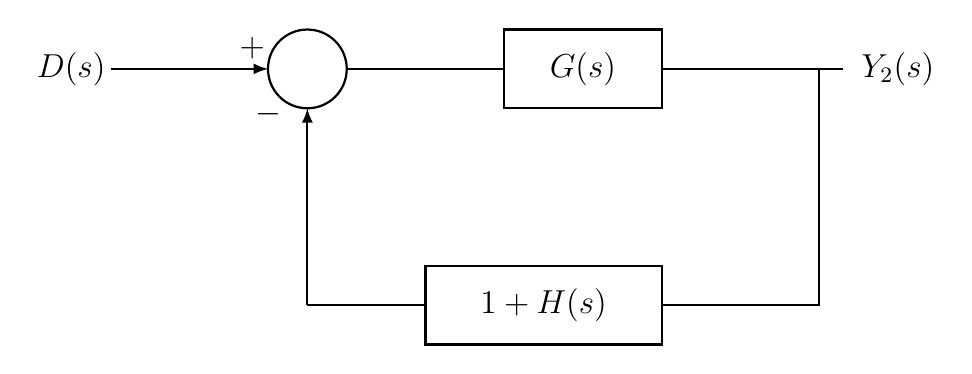
\begin{tikzpicture}[thick, font=\large]
		\draw[-latex] (0,0) -- (2,0);
		\node at (-0.5,0) {$D(s)$};
		\draw (2.5,0) circle[radius=0.5cm];
		\node[above] at (1.8,0) {+};
		\node[below] at (2,-0.3) {$-$};
		\draw[-] (3,0) -- (5,0);
		\draw (5,-0.5) rectangle (7,0.5);
		\node at (6,0) {$G(s)$};
		\draw[-] (7,0) -- (9.3,0);
		\node at (10,0) {$Y_2(s)$};
		\draw[-] (9,0) -- (9,-3) -- (7,-3);
		\draw (7,-3.5) rectangle (4,-2.5);
		\node at (5.5,-3) {$1 + H(s)$};
		\draw[-] (4,-3) -- (2.5,-3);
		\draw[-latex] (2.5,-3) -- (2.5,-0.5);
	\end{tikzpicture}
